%!TEX root = thesis.tex

%:-------------------------- Preamble -----------------------

% Three languages are supported, which will be reflected in the logo on the front page. Pass the appropriate language
% specified as a class option to uit-thesis. Passing any other languages supported by babel will result in the default
% language on the frontpage. If no language is passed, the default is selected.
%  - USenglish (default)
%  - norsk
%  - samin
% The frontpage comes in two variants, Master's thesis and PhD. Master is default, use classoption 'phd' for the PhD version.
\documentclass[USenglish]{uit-thesis}

% Lorem ipsum
\usepackage{lipsum}

\makeglossaries

% Add external glossaryentries
\loadglsentries{acronyms}
\newacronym{api}{API}{application programming interface}\glsunset{api}
\newacronym{2api}{2API}{application programming interface}
\newacronym{d3}{D3}{Data-Driven Documents}
\newacronym{html5}{HTML5}{version 5 of the HyperText Markup Language standard}
\newglossaryentry{thesis}
{
  name=thesis,
  description={is a document submitted in support of candidature for an
    academic degree or professional qualification presenting the author's
    research and findings
    },
}
\newglossaryentry{lage}
{
  name={long ass glossary entry},
  description={is a long ass entry with a lot of text describing the properties of the glossary entry. Hopefully this spans some lines now.
  },
}


\newcommand{\listdefinitionname}{My list of definitions}
\newlistof{definition}{def}{\listdefinitionname}
\newcommand{\definition}[1]{%
  \refstepcounter{definition}%
  \par\noindent\textbf{The Definition~\thedefinition. #1}%
  \addcontentsline{def}{definition}
    {\protect\numberline{\thechapter.\thedefinition}#1}\par%
}

\begin{document}

%:-------------------------- Frontpage ------------------------

\title{Title of the master thesis}
\subtitle{Subtitle}			% Optional
\author{Camilla Stormoen}
\thesisfaculty{Faculty of Science and Technology \\ Department of Computer Science}
\thesisprogramme{Master thesis in Computer Science … May 2018}
%\ThesisFrontpageImage{example_image.jpg}	% Optional

\maketitle

%:-------------------------- Frontmatter -----------------------
\frontmatter

%\begin{dedication}
%To Leslie.
%Fuck you very much.
%\end{dedication}


\begin{epigraph}
\epigraphitem{Simplicity is prerequisite for reliability.}{Edsger Dijkstra}
\epigraphitem{Beware of bugs in the above code;\\I have only proved it correct, not tried it.}{Donald Knuth}
\end{epigraph}


\begin{abstract}
What is wrong with the world? Motivation 1-3 sentences, Arch, Des, Imp, Exp 1,2-3 sentences, results and main conclusion.
\end{abstract}

\begin{acknowledgement}
Thank you ....
\end{acknowledgement}

\tableofcontents

\listofdefinition

%:-------------------------- Mainmatter -----------------------
\mainmatter

\chapter{Introduction}
W3, problem definition: This project investigated .... x, with the purpose of y.

\section{Motivation}

\section{Contributions}

\section{Assumptions}
Avgrense viktig!

\section{Limitations}
Avgrense viktig!
%\paragraph{A paragraph}

\iffalse
\subsection{A subsection}

We can use the \ac{api} to \ac{2api} do stuff, and write about what we did in a \gls{thesis}!

This is some stuff, {\sc smallcaps {\em smallcapsemphasized}} {\em regularemphasized}

\Gls{lage}: a test glossary entry.

If the acronym \ac{uit} is displayed, then loadglsentries works.

It is fun to use modern \upsc{OpenMP} technology!\footnote{This is a snarky
footnote. Words and etc. Semantic web technologies are technologies that enable
semantification of the Web as we know it today. Hopefully this spans some lines
now.}

It is fun to use \emph{modern \upsc{OpenMP}} technology! And it is fun to use \ac{d3} and \ac{html5}.

Referencing figure \ref{fig:ex} to test link.\footnote{This is another
footnote.}

\definition{Some other definition}

\begin{figure}
\centering
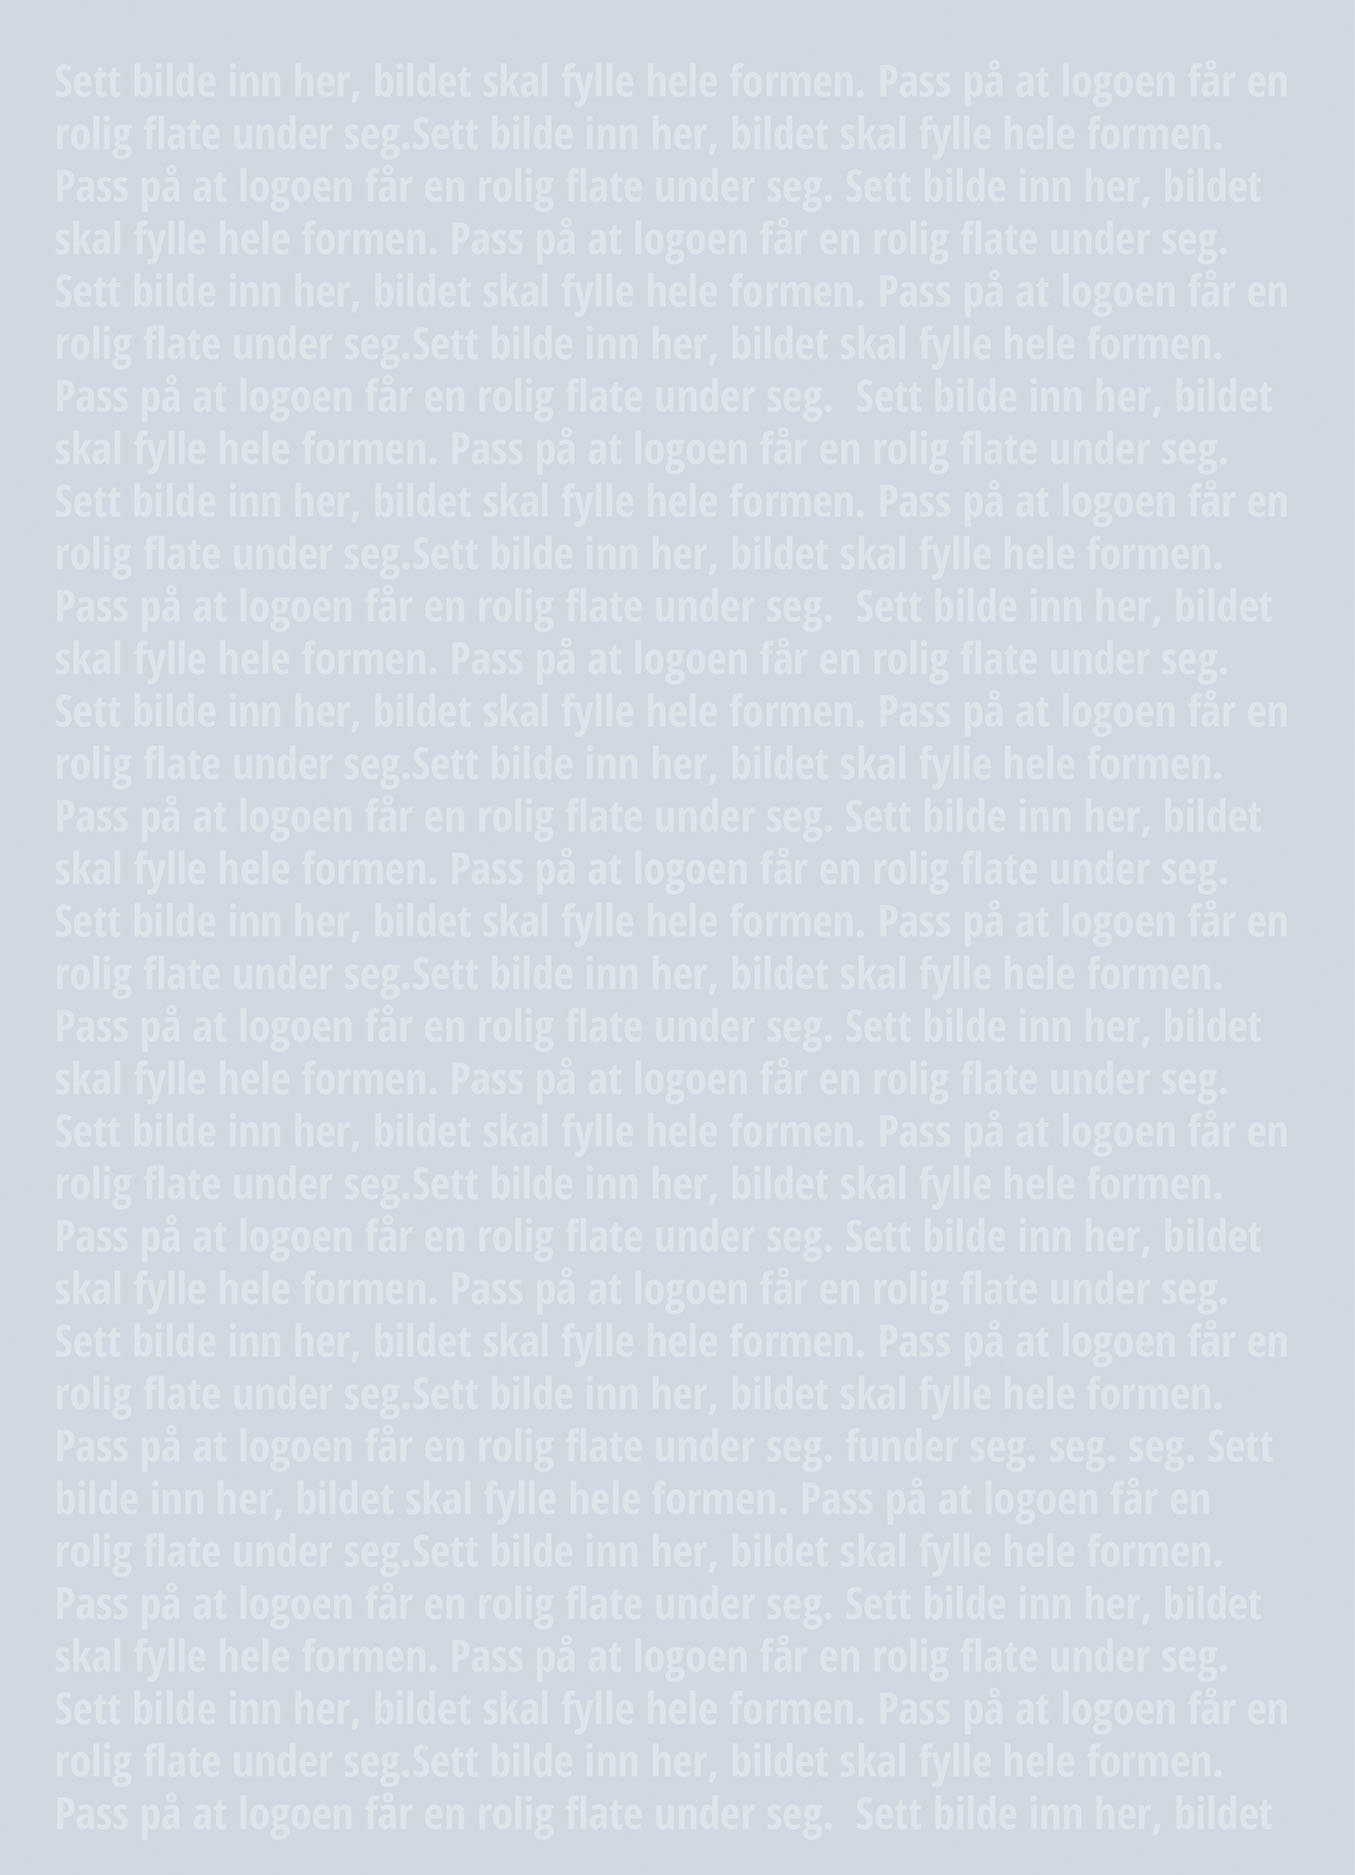
\includegraphics[scale=0.1]{example_image.jpg}
\caption{Figure link should point to top of figure.}
\label{fig:ex}
\end{figure}

\fi


\chapter{Related Work}

\chapter{The Data Set/Background stuff..}

\chapter{Architecture}
Tell it clean/neat. Abstractions, functionalities

\chapter{Design}
Server, p2p, protocols..

\iffalse
\definition{Another definition}

\begin{table}
\centering
\begin{tabular}{|l|l|}
\hline
Content left & Content right\\
\hline
\end{tabular}
\caption{A table}
\end{table}

\begin{table}
\centering
\begin{tabular}{|l|l|}
\hline
Content left & Content right\\
\hline
\end{tabular}
\caption{Another table}
\end{table}

\newpage

\begin{lstlisting}[frame=single,caption={Small C program},language=C]
#include "stdio.h"
#define e 3
#define g (e/e)
#define h ((g+e)/2)
#define f (e-g-h)
#define j (e*e-g)
#define k (j-h)
#define l(x) tab2[x]/h
#define m(n,a) ((n&(a))==(a))

long tab1[]={ 989L,5L,26L,0L,88319L,123L,0L,9367L };
int tab2[]={ 4,6,10,14,22,26,34,38,46,58,62,74,82,86 };

main(m1,s) char *s; {
  int a,b,c,d,o[k],n=(int)s;
  if(m1==1){ char b[2*j+f-g]; main(l(h+e)+h+e,b);
    printf(b); }
  else switch(m1-=h){
    case f:
      a=(b=(c=(d=g)<<g)<<g)<<g;
      return(m(n,a|c)|m(n,b)|m(n,a|d)|m(n,c|d));
    case h:
      for(a=f;a<j;++a)
        if(tab1[a]&&!(tab1[a]%((long)l(n))))
          return(a);
    case g:
      if(n<h)return(g);
      if(n<j){n-=g;c='D';o[f]=h;o[g]=f;}
      else{c='\r'-'\b';n-=j-g;o[f]=o[g]=g;}
      if((b=n)>=e)
        for(b=g<<g;b<n;++b)o[b]=o[b-h]+o[b-g]+c;
      return(o[b-g]%n+k-h);
    default:
      if(m1-=e) main(m1-g+e+h,s+g); else *(s+g)=f;
      for(*s=a=f;a<e;) *s=(*s<<e)|main(h+a++,
      (char *)m1);
    }
}
\end{lstlisting}

\fi


\chapter{Implementation}
Threads, data structures, language

\chapter{Evaluation}
\section{Experimental Setup}
\section{Experimental Design}
\section{Results}
What does the results say?
\subsection{Result 1}


\chapter{Discussion}
Idea, arch, design, resutls, other solutions, "arch has scale issue"

\chapter{Conclusion}

\chapter{Future Work}

\chapter{Appendix}


\backmatter

%%% BIBLOGRAPHY

\newpage{}

\begin{thebibliography}{9}
%1
%\bibitem{VirtualSensors2006}
%S. Kabadayi and A. Pridgen and C. Julien,
%\newblock {\em Virtual Sensors: Abstracting Data from Physical Sensors}, 2006,
%\newblock in {\em 2006 International Symposium on a World of Wireless, Mobile and Multimedia Networks(WoWMoM'06), 6 pp.-592}.

\end{thebibliography}


\end{document}

